\chapter{Анализ данных эксперимента}

После проведения экспериментальных исследований влияния радиуса закругления рабочей кромки и шага резания на составляющие силы, возникающей на дисковом инструменте, при механическом разрушении льда получен набор <<сырых>> данных, который включает в себя:
\begin{itemize}
	\item фотографии осколков;
	\item графики переходных процессов для каждого сочетания факторов.
\end{itemize}

Дальнейшее их использование предполагает обработку и оценку корректности методами математики и статистики, такими как:
\begin{itemize}
%	\item оценка дисперсии;
	\item усреднение значений;
	\item фильтрация постоянной составляющей;
	\item отброс грубых ошибок;
	\item сглаживание.
\end{itemize}

Далее в это главе процесс обработки и оценки адекватности данных будет приведен последователь.

\section{Фильтрация и сглаживание переходных процессов резания льда}

Чтобы исключить <<дрейф нуля>> необходимо убрать из сигнала переходного процесса постоянную составляющую. Самый простой способ это сделать, перевести сигнал в частотную область (например быстрым преобразованием Фурье (БПФ)) \cite{BPF,BPFEng}. Воспользуемся следующей формулой для реализации БПФ:
\begin{equation}\label{eq:FFT}
X(k)=\sum_{j=1}^{N} x(j)\cdot\omega_{N}^{(j-1)\cdot(k-1)}
\end{equation}
где $ N $ "--- количество точек в снятом переходном процессе; $ \omega_{N} = e^{\frac{-2\pi i}{N}} $ "--- корень $ N $-ой степени.

После перехода в частотную область, сигнал представляет собой значение частот всех гармоник образующих исходный сигнал. Можно графически оценить полученную спектрограмму, рисунок \ref{img:Spectrum}. Как известно из главы \ref{chapt2}, частота дискретизации АЦП равна 100~Гц. На графике же мы видем максимальную частоту 50~Гц, это обусловленно линейностью и симметричностью преобразования Фурье. 
\begin{figure}[ht] 
	\center
	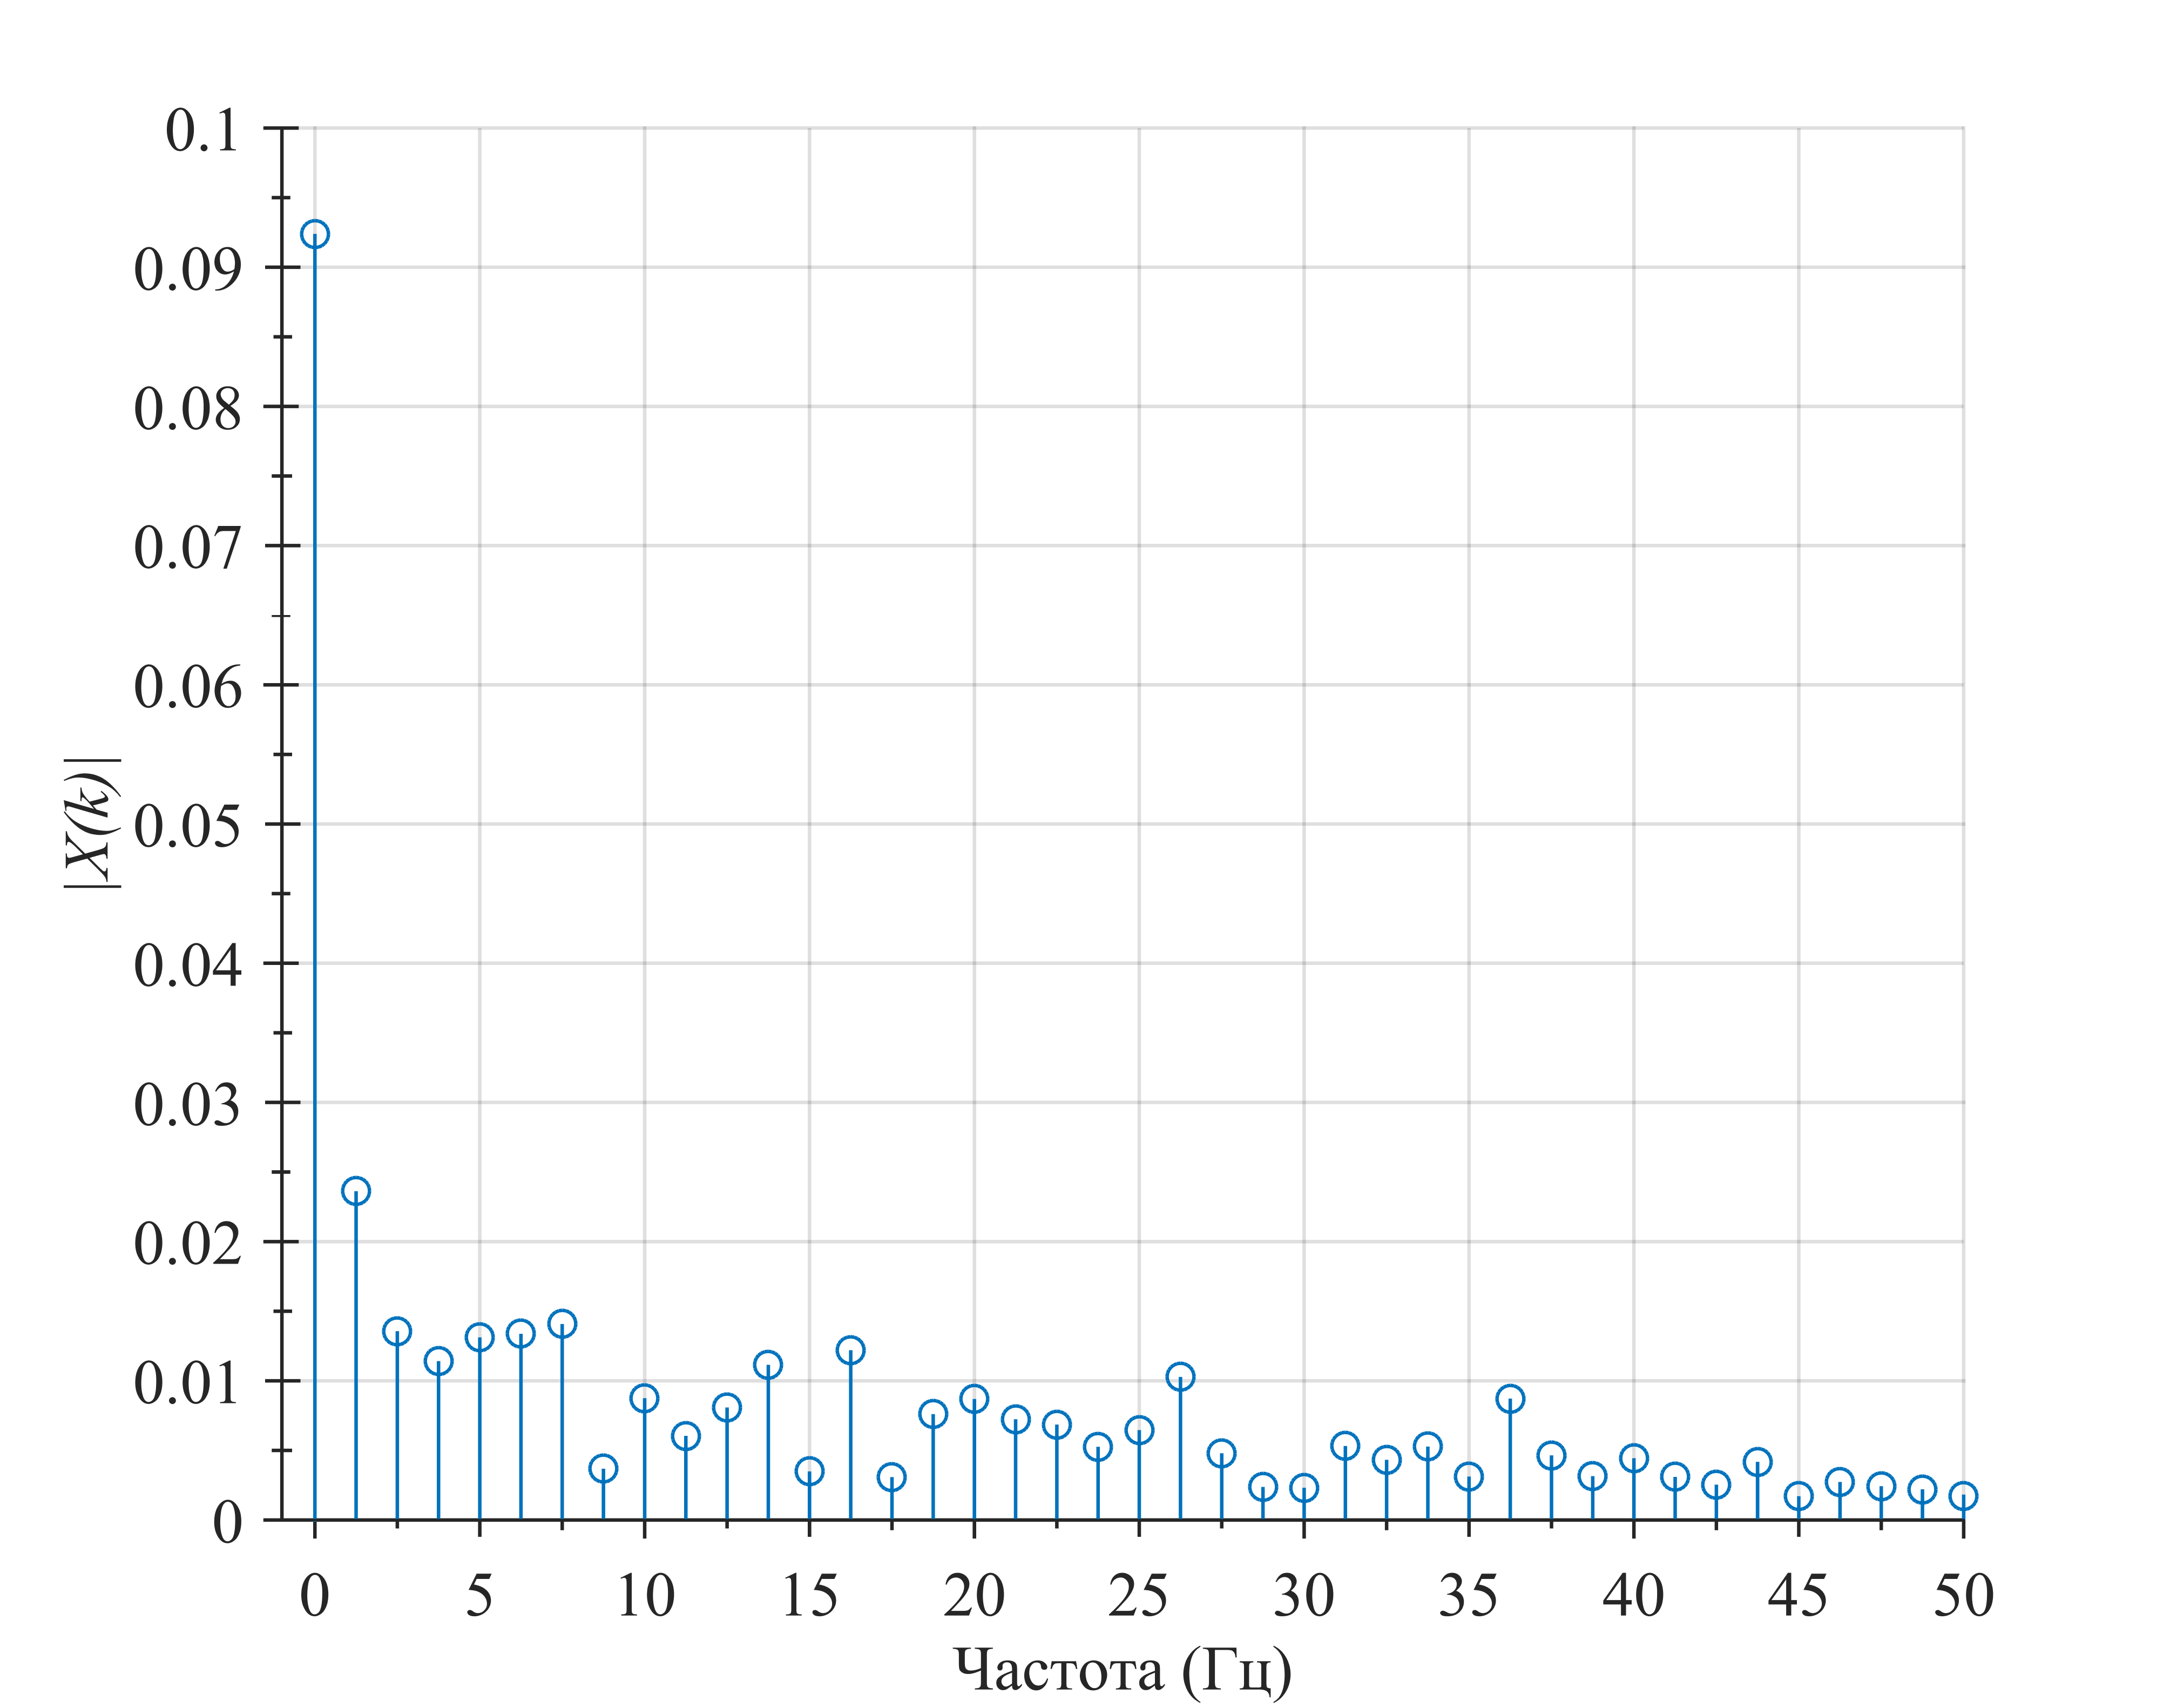
\includegraphics{Spectrum}
	\caption{Спектрограмма сигнала переходного процесса разрушения льда} 
	\label{img:Spectrum}  
\end{figure}

Как видно из рисунка \ref{img:Spectrum} на нулевой частоте заметен значительный всплеск амплитуды. Что обуславливает присутствие в сигнале некой постоянной составляющей с амплитудой равной 0,185. 0.0792  Для удаления постоянной составляющей сигнала достаточно просто обнулить нулевую частоту в полученно ряду Фурье и выполнить обратное преобразование с помощью формулы \ref{eq:iFFt}

Обратное преобразование будет иметь вид:
\begin{equation}\label{eq:iFFT}
x(j)=\frac{1}{N}\sum_{k=1}^{N} X(k)\cdot\omega_{N}
\end{equation}

Приведем пример <<сырого>> сигнала переходного процесса, рисунок \ref{img:SignalRaw} синяя линия. Также на рисунке \ref{img:SignalRaw} изображен сигнал полученный путем отбрасывания нулевой частотной составляющей в ряду Фурье
\begin{figure}[ht] 
	\center
	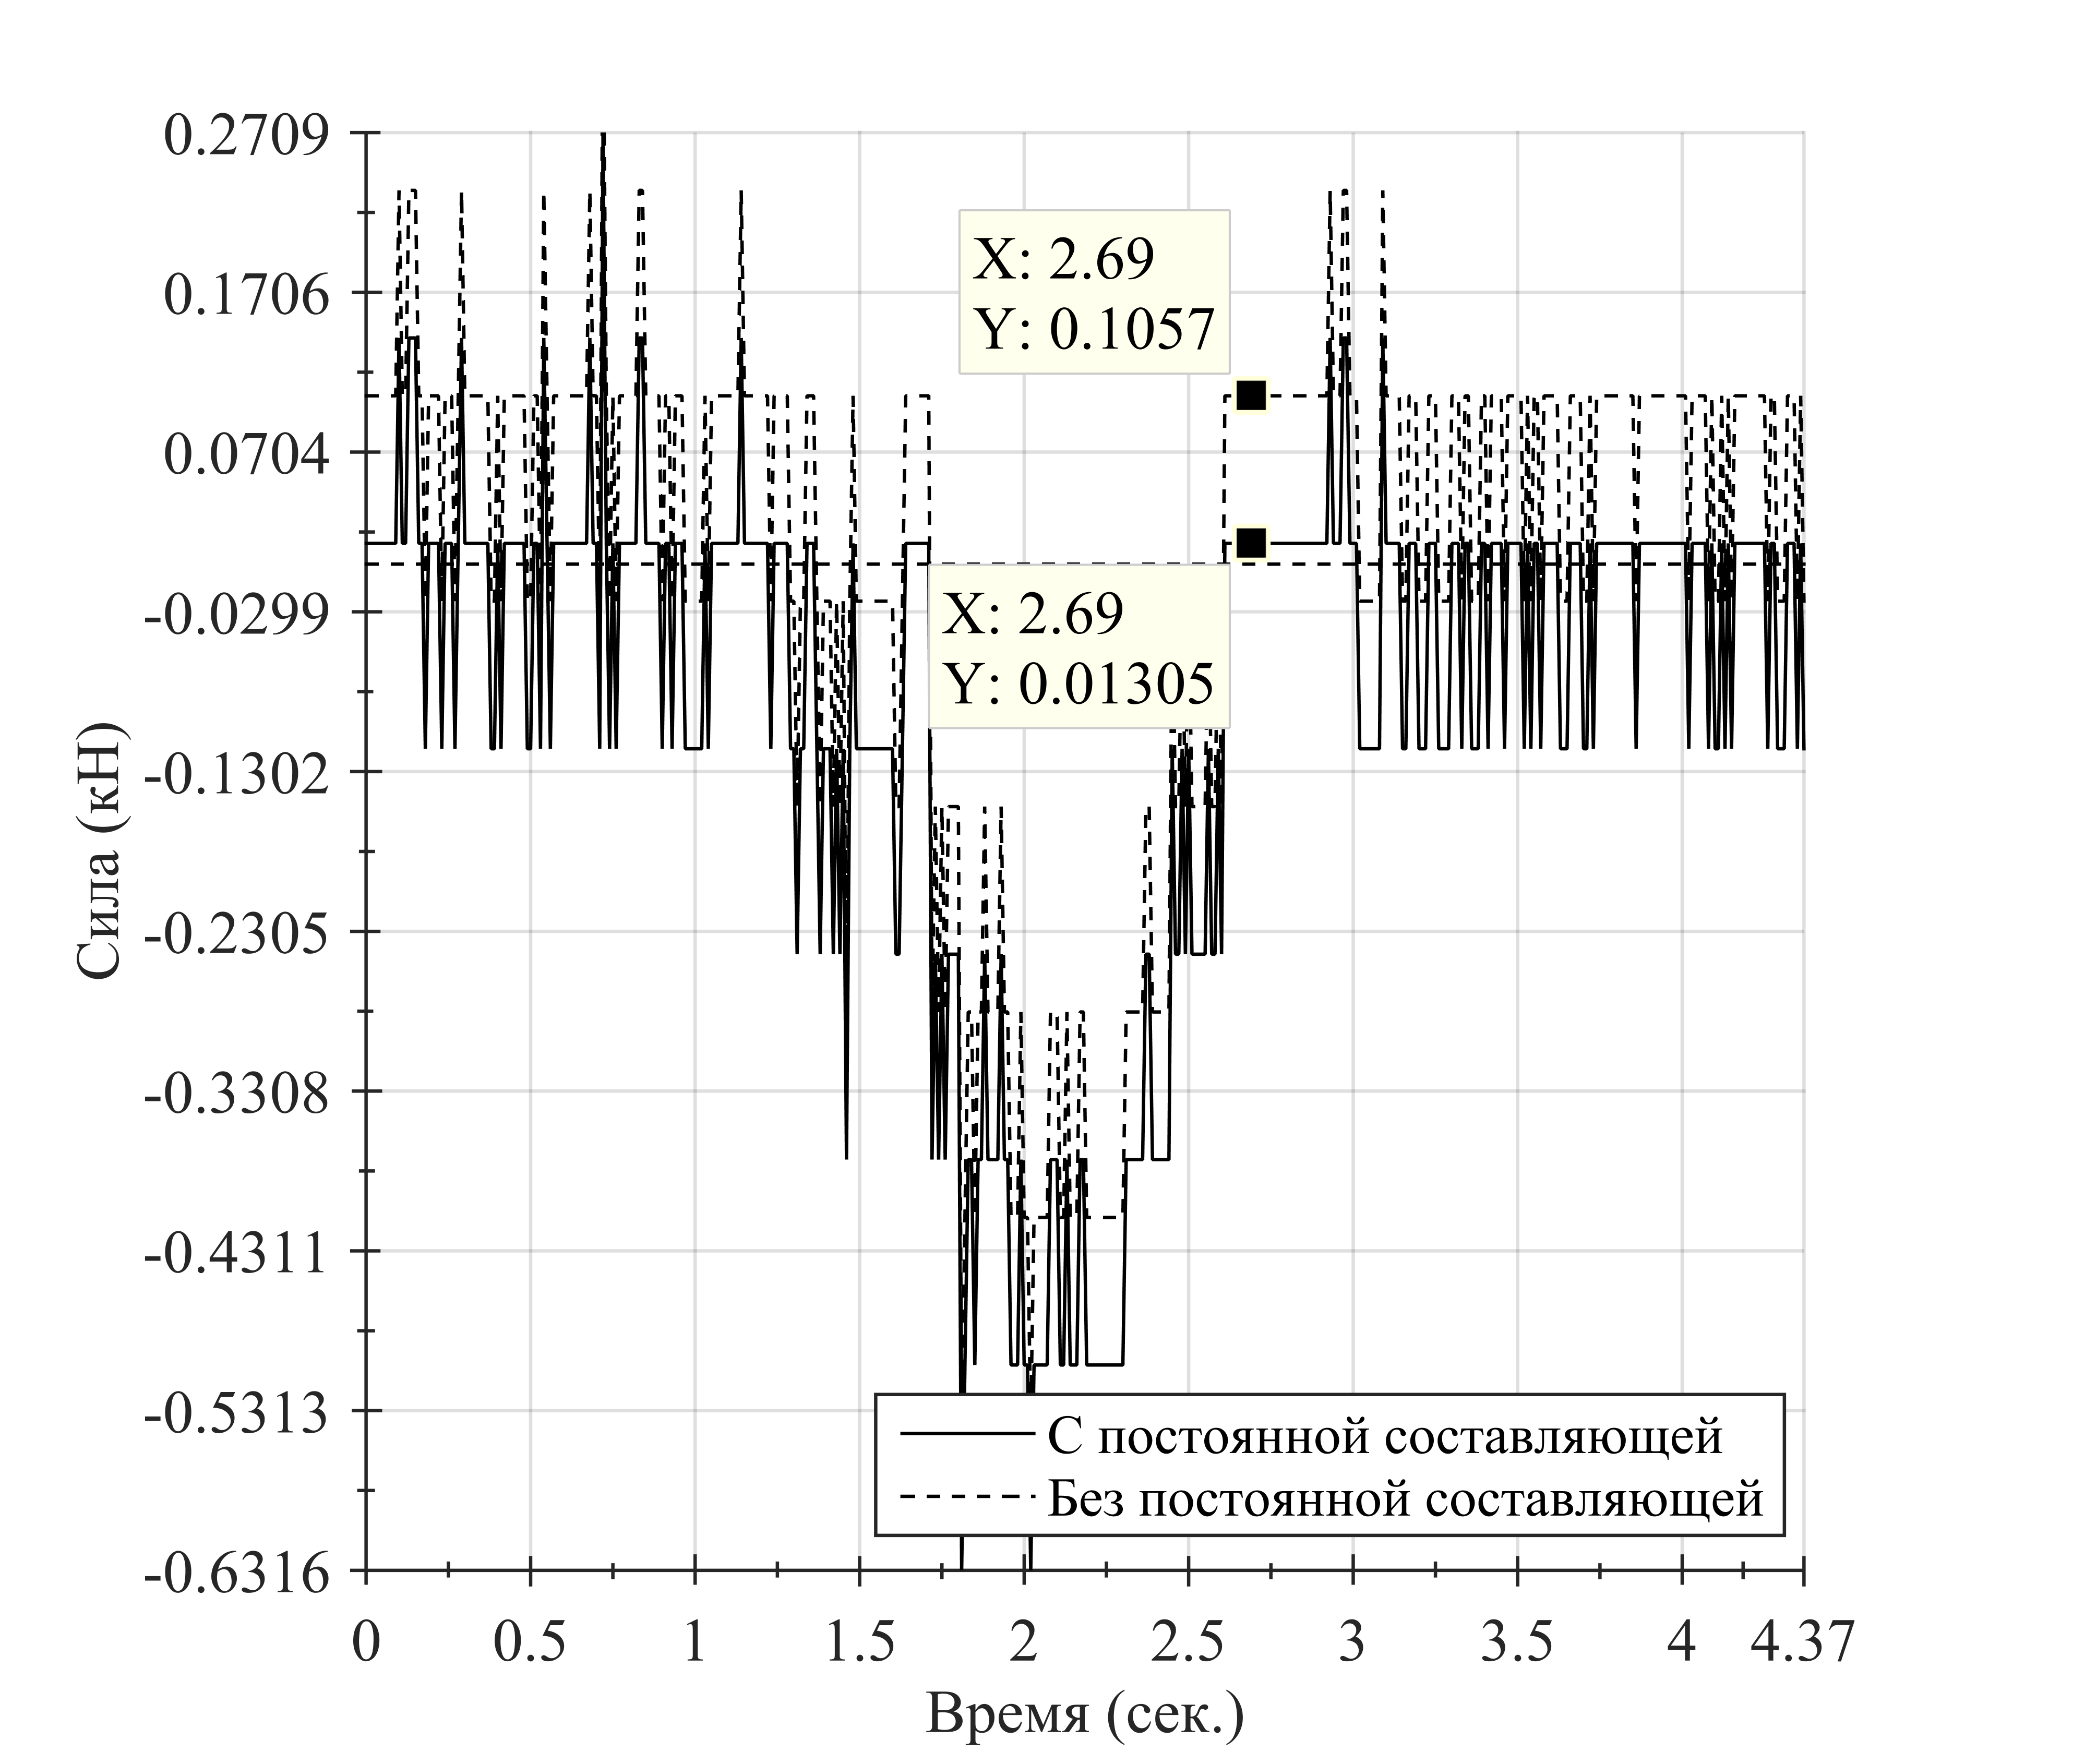
\includegraphics{SignalRaw}
	\caption{Переходный процесса разрушения льда} 
	\label{img:SignalRaw}  
\end{figure}



\section{Усреднение повторных опытов}

Из параграфа \ref{sect2_2} известно, что для каждый опыт повторялся 5 раз, для учета неизвестных факторов, а это значит что данные необходимо усреднить.

Точечную оценку величины действующей силы можно вычислить через:
\begin{equation}\label{eq:x_ocenka}
\hat{a}=\frac{1}{n}\sum_{i=1}^{n} F_i,
\end{equation}
где $ n $ "--- число повторных опытов, $ F_i $ "--- измеренное значение в отдельном опыте \cite{Zajigaev}.

Среднеквадратичное отклонение точечной оценки 
Оценить точность позволит относительная погрешность измерений, вычисляемая по следующее формуле:
\begin{equation}\label{eq:Error}
\varepsilon=\frac{1}{n}\sum_{i=1}^{n} \frac{\left| x_i-\bar{x}\right| }{\bar{x}}\cdot100\%
\end{equation}